\section{Motivation}
\begin{frame}{Motivation}
	\begin{itemize}
		\item Phenomenology of NP models depends on free parameters \\{\footnotesize(e.g. points in the space of Wilson coefficients)}
		\item Influences shape of kinematic distributions
	\end{itemize} 
	
	\bigskip
	\stress{Problems:}
	\begin{itemize}
		\item Need to make assumptions on kinematic distributions for predictions and measurements\\
		$\Lra$ Need to re-run analysis for different NP models and their parameters
		\item Difficult to present numeric results (e.g. exclusion limits)\\
		{\footnotesize (there are no nice ways to visualize 3+ dimensions)}\\
		%\item Difficult to evaluate sensitivity to NP parameters
	\end{itemize}
\end{frame}
%
\begin{frame}[t]{Motivation II}{Example}
	\mauthor{BaBar}'s result for $R(D^{(*)})$ based on model assumption\\
	{\footnotesize(2HDM with specific $\tan\beta$ parameter)}\\
			
	\medskip
	\begin{center}
	\only<1>{
		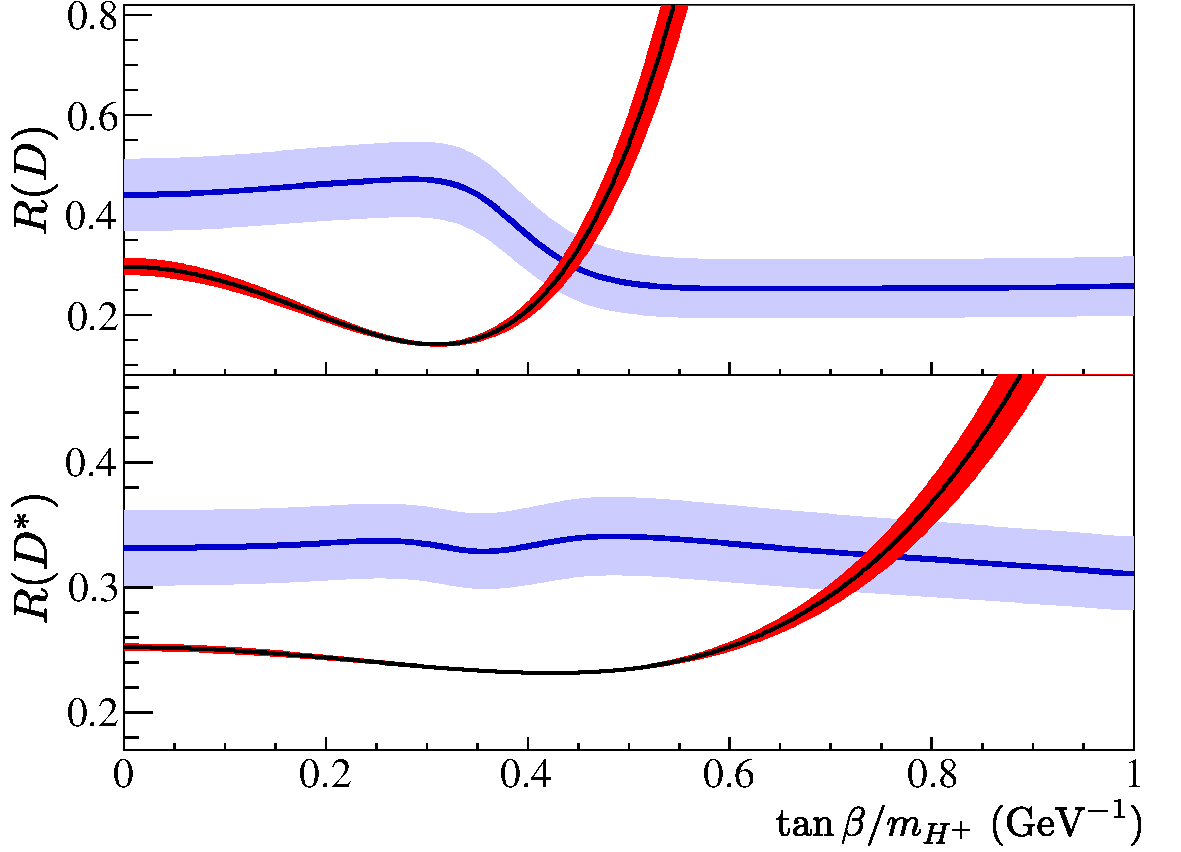
\includegraphics[width=7cm]{figures/type2_2hdm_vs_rd_rds_1205_5442.pdf}	
	}
	\only<2>{
		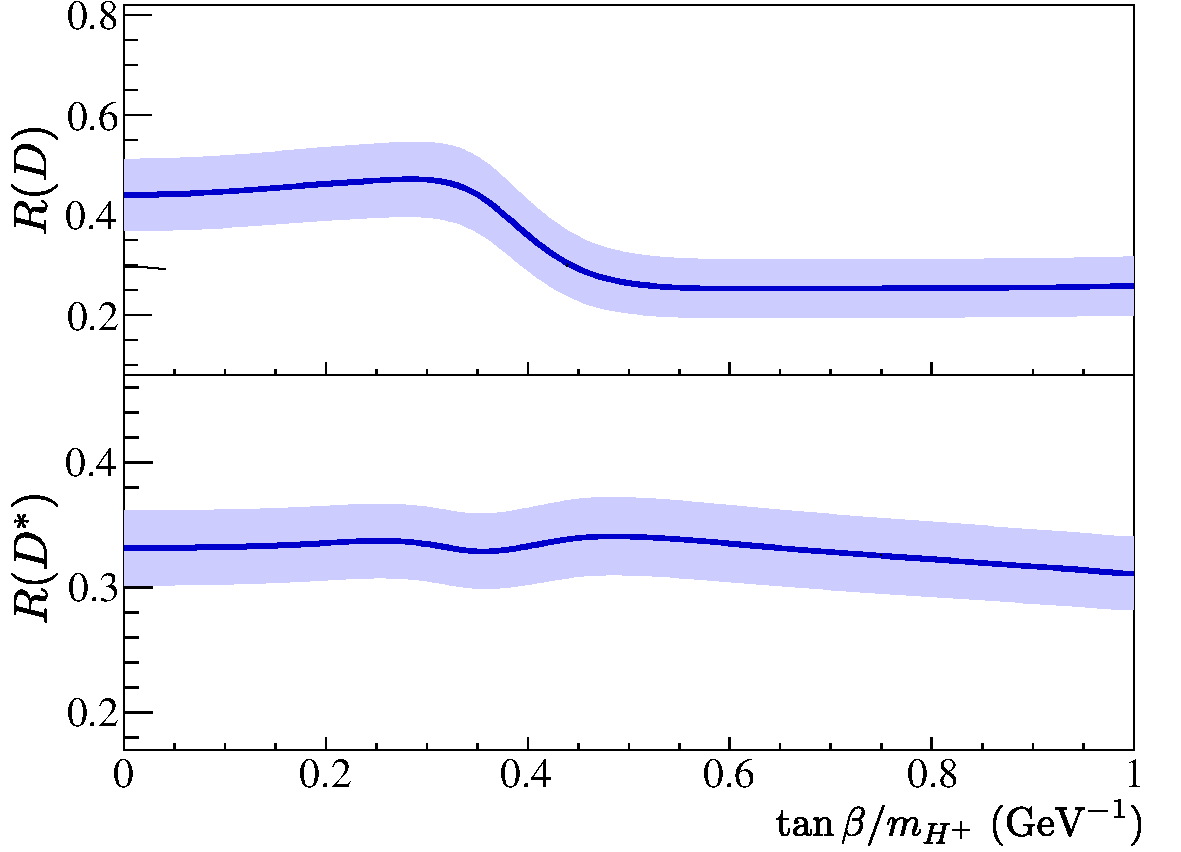
\includegraphics[width=7cm]{figures/type2_2hdm_vs_rd_rds_1205_5442_results_only.pdf}\\[1ex]
		Results obtained from a 2D fit to $m_\text{miss}^2$ and $|\vec p_\ell|$
	}
	\only<3>{
		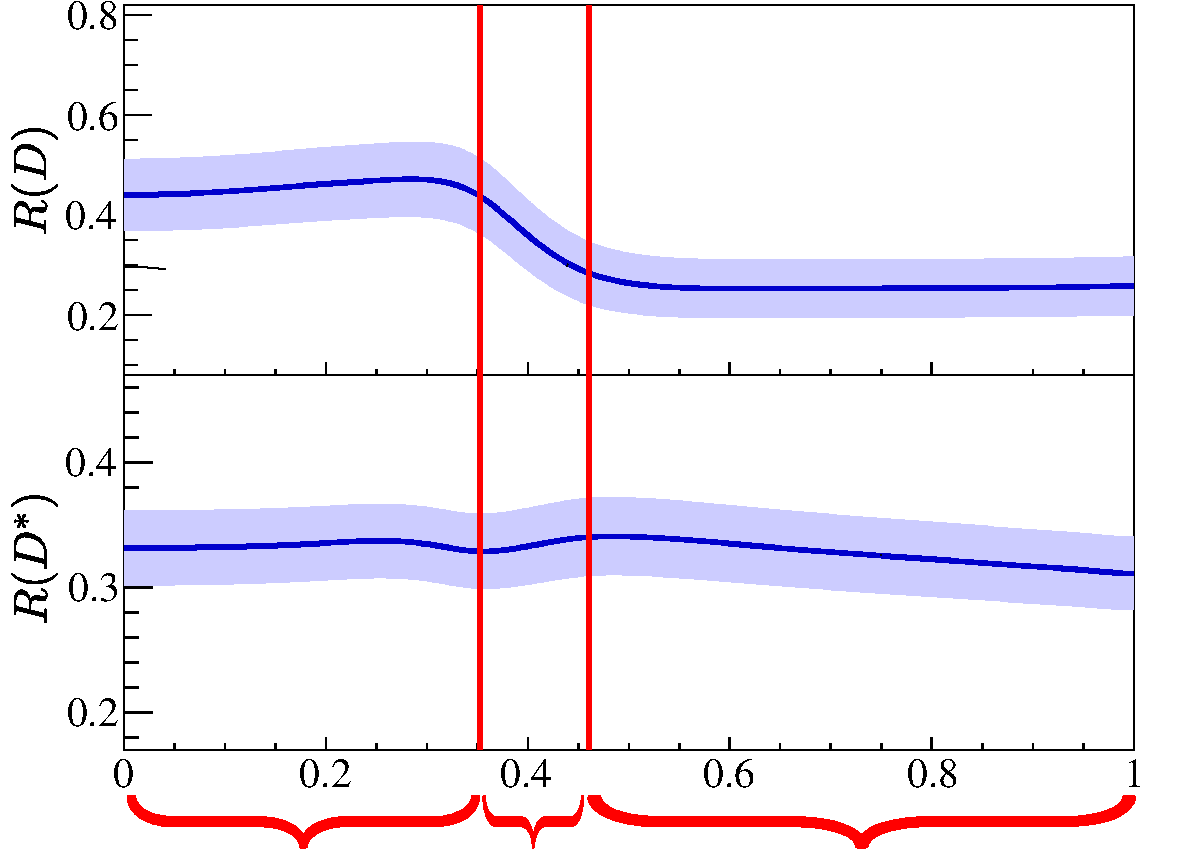
\includegraphics[width=7cm]{figures/type2_2hdm_vs_rd_rds_1205_5442_results_only_cluster.pdf}\\[1ex]
		\begin{changemargin}{-0.25cm}{-0.25cm}
			\small
			In the three parts, the $m_\text{miss}^2$--$|\vec p_\ell|$  behavior of the model has probably been different $\Lra$ Would have been nice to categorize the parameter space by this behavior right away
		\end{changemargin}
	}
	\end{center}
\end{frame}
%
\begin{frame}{Motivation III}
	\large
	\stress{Clustering}: \\[1ex]
	\badc{\textbf{Multi-dimensional parameter space}} $\longrightarrow$ \goodc{\textbf{few benchmark points}}!
	
	\bigskip
	Particular use case: Cluster \stress{kinematic distributions} in space of \stress{Wilson coefficients}.
\end{frame}
%
%\begin{frame}{Clustering of $B\lra D^{(*)} l \nu$ kinematic shapes}
%	\textbf{Team:}
%	\begin{itemize}
%		\item Original idea/kickoff/implementation of distributions: \mauthor{Alejandro Celis} \\
%		(left in November 2018) 
%		\item Open development on \url{https://github.com/RD-clustering/B_decays_clustering/}
%		\item Also on board: \mauthor{Jason Aebischer}
%	\end{itemize}
%	\textbf{Problem:} Phenomenology of NP models depends on free parameters influencing the shape of kinematic distributions $\Lra$
%	\begin{itemize}
%		\item Difficult to present exclusion limits
%		\item An issue for analyses that need to make assumptions on kinematic distributions to extract features of interest (but still want to publish their results in a very general way)
%	\end{itemize}
%	\textbf{Solution:}
%	\begin{itemize}
%		\item Cluster NP parameter space based on a metric quantifying similarity of the result kinematic distributions
%		\item Choose NP benchmark point representing each cluster cluster
%		\item Report exclusion limits and measurements for each benchmark point
%	\end{itemize}
%\end{frame}
%%
%%
%\begin{frame}
%	\textbf{Examples:}
%	\begin{itemize}
%		\item For 2HDMs: \reference{https://arxiv.org/abs/1507.02245}{1507.02245} (used by \mauthor{ATLAS} and \mauthor{CMS})
%		\item Example of the dependency of result based on hypothesis (\mauthor{BaBar}):\\
%		
%		\medskip
%		{\centering
%			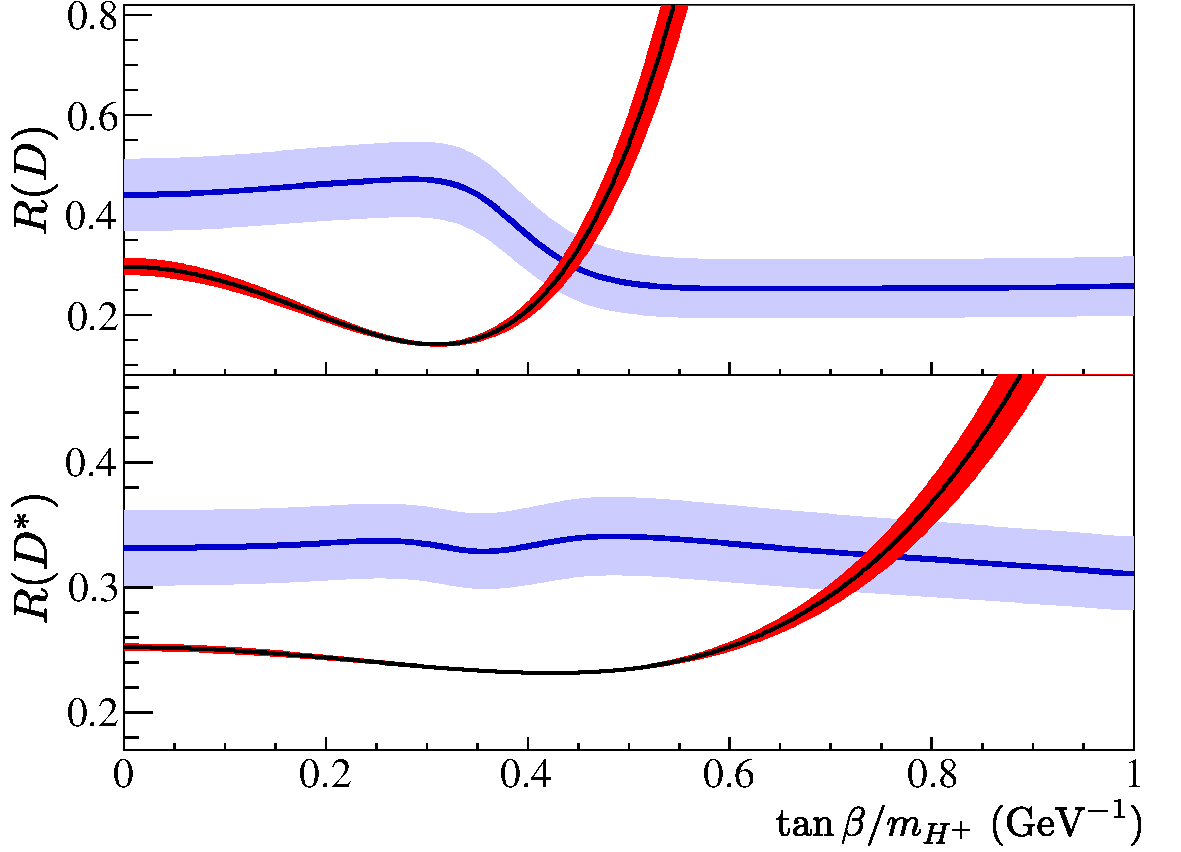
\includegraphics[width=8cm]{figures/type2_2hdm_vs_rd_rds_1205_5442.pdf}	
%			\par
%		}
%	\end{itemize}
%\end{frame}